The platform's primary metadata, user information, and agent configurations are stored in a relational database managed by Supabase, which runs on PostgreSQL. The logical structure of this database is represented by the physical \ac{er} diagram shown in Figure~\ref{FIG:ER_DIAGRAM}. This schema is designed to efficiently store and retrieve information about users, the agents they create, and their conversation histories, while also implementing specific workarounds for the platform's real-time features.

\begin{figure}[Entity-Relationship Diagram]{FIG:ER_DIAGRAM}{\ac{er} Diagram for the Metadata Database.}
    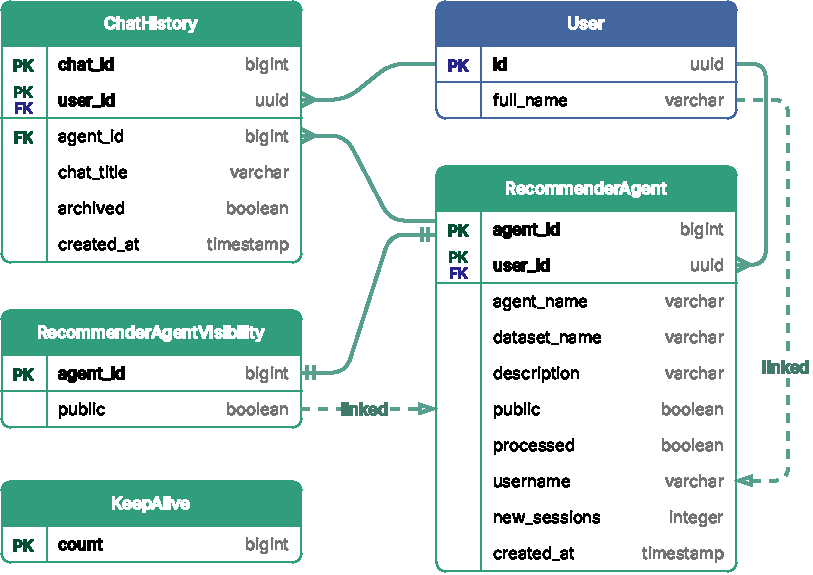
\includegraphics[width=0.9\textwidth]{er_diagram.pdf}
\end{figure}

The core entities are defined as follows:
\begin{compactitem}[\textbullet]
    \item \textbf{User:} This entity is implicitly managed by Supabase's built-in \texttt{auth.users} table. It is not defined directly in the public schema but is referenced via a \texttt{user\_id} foreign key in other tables, linking data to a specific authenticated user.
    \item \textbf{RecommenderAgent:} This is the central table for storing all metadata associated with a created agent. It includes attributes such as the agent's name, the dataset it was trained on, its description, its processing status, and its visibility (public or private). Additionally, \texttt{new\_sessions} tracks the number of new conversations users had with an agent since its last retraining, as an indicator of the agent's engagement for the creator. Each agent is directly linked to a creator via the \texttt{user\_id}, and the user's username is also duplicated for public visibility.
    \item \textbf{RecommenderAgentVisibility:} This auxiliary table was created to address a specific challenge with Supabase's real-time capabilities. When \acl{rls} is active, the frontend cannot listen for real-time changes on rows that a user does not have access to (e.g., when an agent becomes private). This table, which is fully public, mirrors the \texttt{agent\_id} with a foreign key and the \texttt{public} status with an automatic trigger, allowing the frontend to subscribe to its changes and correctly update the \acs{ui} when an agent's visibility changes.
    \item \textbf{ChatHistory:} This table archives the records of conversations. Each entry is linked to a \texttt{user\_id}, and optionally to an \texttt{agent\_id} (which is \texttt{null} for Open Chat histories), storing the conversation title and an \texttt{archived} flag to distinguish active from read-only sessions.
    \item \textbf{KeepAlive:} A utility table with a single auto-incrementing counter. Its sole purpose is to be updated by a scheduled daily job to prevent the database from being paused by Supabase's inactivity policy.
\end{compactitem}
